\chapter{Check routines}
\section{Introduction}
This chapter describes the routines that can be used to check the design following the specifications of different design codes.

\section{Check routines for steel}

\subsection{Lateral torsional buckling of steel beams (EC3)}
Flexural buckling check, according to article 5.5.2 of EC3, can be written as:

\begin{equation}
F= \frac{M_d}{M_{b,Rd}} \leq 1
\end{equation}   

\noindent where:
\begin{description}
\item{$M_d$} Design value of bending moment.
\item{$M_{b,Rd}$} Buckling resistance
\end{description}

\subsubsection{Design lateral torsional buckling resistance $M_{b,Rd}$}
Design value of lateral torsional buckling resistance can be determined as follows:

\begin{equation}
M_{b,Rd}= \chi_{LT} \cdot W_y \cdot \frac{f_y}{\gamma_{M1}} 
\end{equation}

\noindent where $\gamma_{M1}$ is the partial factor for member buckling resistance and $f_y$ is the characteristic value of the yield strength.

\paragraph{Cross section modulus $W_y$}
\begin{equation}
W_y= \left\{
\begin{array}{lr}
W_{pl,y} & : \text{1 or 2 class cross section (plastic section modulus)}\\
W_{el,y} & : \text{class 3 cross section (elastic section modulus)}\\
W_{eff,y} & : \text{class 4 cross section (effective section modulus)}
\end{array}
\right.
\end{equation}

\paragraph{Reduction factor $\chi_{LT}$}
The reduction factor $\chi_{LT}$ for the appropriate non-dimensional slenderness $\lambda_{LT}$ may be determined from:

\begin{equation}
\chi_{LT}= \frac{1}{\phi_{LT}+\sqrt{\phi_{LT}^2-\overline{\lambda}_{LT}^2}}
\end{equation}

\subparagraph{Intermediate factor $\phi_{LT}$} calculated as:

\begin{equation}
\phi_{LT}= 0.5 [1+\alpha_{LT}\cdot(\overline{\lambda}_{LT}-0.2)+\overline{\lambda}_{LT}^2]
\end{equation}

\subparagraph{Imperfection factor $\alpha_{LT}$}
Depending on the buckling curves \footnote{Selection of flexural buckling curve for a cross section can be made from EC3 tables.}:

\begin{equation}
\alpha_{LT}= \left\{
\begin{array}{lr}
0.21 & : \text{curve a}\\
0.34 & : \text{curve b}\\
0.49 & : \text{curve c}\\
0.76 & : \text{curve d}
\end{array}
\right.
\end{equation}

\subparagraph{Non-dimensional beam slenderness $\overline{\lambda}_{LT}$} calculated as:

\begin{equation}
\overline{\lambda}_{LT}= \sqrt{\frac{W_y f_y}{M_{cr}}}
\end{equation}

Where the non-dimensional slenderness $\overline{\lambda}_{LT} \leq 0.4$ no allowance for lateral-torsional buckling is necessary\footnote{This value can be adapted in the national annex.}

\subparagraph{Critical bending moment $M_{cr}$}
Following the \cite{lopez06} reference, the elastic critical moment is directly affected by the following factors:

\begin{itemize}
\item Material properties (elastic modulus, poisson ratio,\ldots).
\item Properties of the cross section (torsion constant, warping constant\footnote{The effect of torsional loading can be split into two parts, the first part causing twist and the second, \emph{warping}.} and moment of inertia about the minor axis).
\item Properties of the beam such as its length, lateral bending and warping restrictions at supports.
\item Loading: lataeral-torsional buckling is greatly affected by moment diagram and loading position with respect to the section shear centre.
\end{itemize}

\begin{figure}
\centering
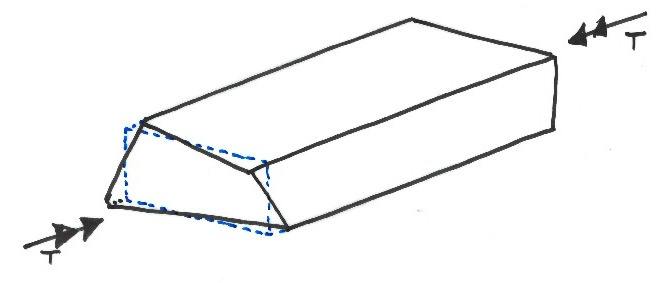
\includegraphics[width=90mm]{materials/figures/warping}
\caption{Warping on a rectangular section due to pure torsion}\label{fg_warping}
\end{figure}

As a generally accepted procedure, consideration of the bending moment diagram is taken into account by means of the \emph{equivalent uniform moment factor (EUMF)}, also called the \emph{moment gradient correction factor}. The elastic critical moment for any bending moment diagram is obtained by multipliying this factor by the elastic critical moment of the simply supported beam with uniform moment.

The expression of the elastic critical moment is the calculated as:

\begin{equation}
M_{cr}= C_1 \frac{\pi^2 EI_z}{(k_z L)^2} \sqrt{(\frac{k_z}{k_w})^2 \frac{I_w}{I_z}+\frac{(k_z L)^2 GI_t}{\pi^2 EI_z}} 
\end{equation}

\noindent where the lateral bending coefficient $k_z$ and the warping ceofficient $k_w$ are introduced to consider support conditions different from the simply supported beam. These coefficients are equal to 1 for free lateral bending and free warping and 0.5 for prevented lateral bending and prevented warping. There rest of the parameters are defined as follows:

\begin{description}
\item{$E$} Elastic modulus.
\item{$G$} Shear modulus.
\item{$k_z L$} Lateral torsional buckling length of the beam: length between points which have lateral restraint.
\item{$I_z$} Moment of inertia about the minor axis.
\item{$I_t$} Torsional constant.
\item{$I_w$} Warping constant.
\end{description}

Finally, the moment moment gradient factor $C_1$ is calculated as:

\begin{equation}
%%\frac{
C_1= \frac{\sqrt{\sqrt{k} A_1+[\frac{(1-\sqrt{k})}{2} A_2]^2}+\frac{(1-\sqrt{k})}{2} A_2}{A_1}
\end{equation}

\noindent where:
\begin{description}
\item{$k= \sqrt{k_1 k_2}$} depends on the lateral bending and warping conditions coefficients $k_1$ and $k_2$.
\item{$M_i$ and $M_{max}$} moments which represent moment diagram of the beam as in figure \ref{fg_moment_diagrams}. $M_{max}$ is the maximum moment and $M_1$, $M_2$, $M_3$, $M_4$ and $M_5$ are the values of the moment at the different sections of the beam as indicated int the figure, each of them wit the corresponding sign.
\item{$A_1= \frac{M_{max}^2+\sum\limits_{i= 1..5} \alpha_i M_i^2}{(1+\sum\limits_{i= 1..5} \alpha_i) \cdot M_{max}^2}$}
\item{$A_2= \frac{M_1+2 M_2+ 3 M_3 + 2 M_4 + M_5}{9 \cdot M_{max}}$}
\item{$\alpha_i$} factor calculated as follows:
\begin{equation}
\alpha_1= (1-k_2);\ \alpha_2= 5 \frac{k_1^3}{k_2^2};\ \alpha_3= 5 (\frac{1}{k_1}+\frac{1}{k_2});\ \alpha_4= 5 \frac{k_2^3}{k_1^2};\ \alpha_5= (1-k_1)
\end{equation}
\item{$k_1$ and $k_2$} support conditions at each end of the beam as follows:
\begin{description}
\item{$k_1= 1.0$} Free lateral bending and warping at left end.
\item{$k_1= 0.5$} Prevented support conditions at left end.
\item{$k_2= 1.0$} Free lateral bending and warping at right end.
\item{$k_2= 0.5$} Prevented support conditions at right end.
\end{description}
\end{description}

\begin{figure}
\centering
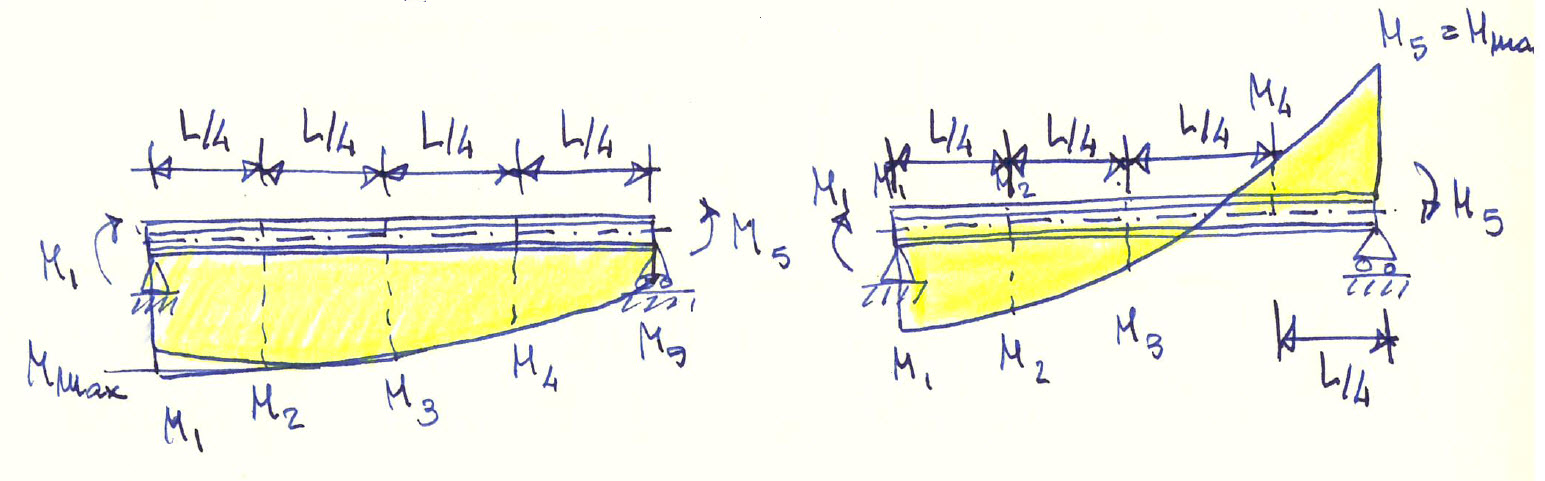
\includegraphics[width=120mm]{materials/figures/ltb_moment_diagrams}
\caption{Moment diagrams and moment values for calculation of $C_1$}\label{fg_moment_diagrams}
\end{figure}

\section{Check routines for reinforced concrete}
\subsection{Verification of RC shell sections}
\subsubsection{Sections definition}
\paragraph{hormigonesEHE}
\begin{verbatim}
from materials.ehe import hormigonesEHE
\end{verbatim}

\paragraph{EHE\_reinforcing\_steel}
\begin{verbatim}
from materials.ehe import EHE_reinforcing_steel
\end{verbatim}

\paragraph{RecordRCSlabSection}
\begin{verbatim}
from materials.fiber_section import defSeccionHASimple
\end{verbatim}


\subsubsection{Types of calculation}
\paragraph{defInteractionDiagram}

\paragraph{simple\_static\_linear}
\begin{verbatim}
from solution import predefined_solutions
predefined_solutions.simple_static_linear
\end{verbatim}

\subsubsection{Limit State at Failure under normal stresses verification}

\paragraph{lanzaCalculoTNFromXCData}
This function carries out the verification of the limit state at failure under nornal stresses. It takes as input the internal forces and bending moments calculated for the shell elements for every ULS combinations, the sections definition and the interaction diagrams to be employed.

The function returns two files with the verification results:
{\tt outputFileName.py}: XC file that assigns each shell element the capacity factor (worst-case) {\tt FCC} calculated for reinforcement in directions 1 and 2, together with the concomitant axial force and bending moments {\tt N My Mz}.
{\tt outputFileName.py}: \LaTeX\  file containing a table with the following items:

\begin{center}
\begin{tabular}{ccccccc}
\multicolumn{7}{l}{\textbf{Section 1}} \\
\\
Element & Section & ULS & Axial & Bending & Bending & Capacity \\
number  & name & name & force NCP1 & moment MyCP1 & moment MzCP1 & factor FCCP1 \\
\hline
\multicolumn{7}{l}{\ldots\ \ldots\ \ldots} \\
\\
\multicolumn{7}{l}{\textbf{Section 2}} \\
\\
Element & Section & ULS & Axial & Bending & Bending & Capacity \\
number  & name & name & force NCP2 & moment MyCP2 & moment MzCP2 & factor FCCP2 \\
\hline
\multicolumn{7}{l}{\ldots\ \ldots\ \ldots} \\
\\

\end{tabular}
\end{center}

\begin{figure}[h]
\centering
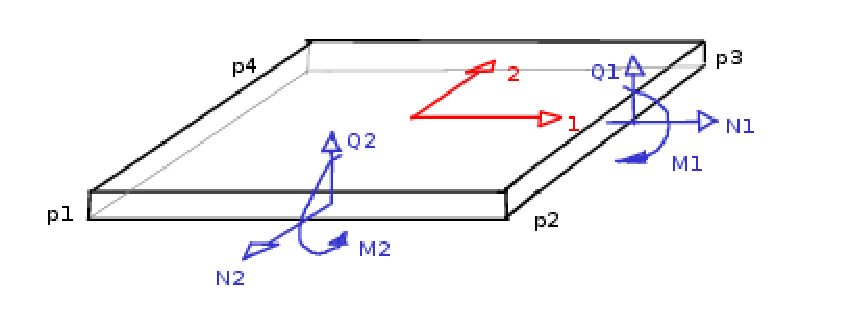
\includegraphics[width=100mm]{materials/figures/signosEsfuerzos}
\caption{Positive directions of forces and moments in shell elements}\label{shell_forces_moments}
\end{figure}

 
\begin{verbatim}
from materials.xLamina import calculo_tn
calculo_tn.lanzaCalculoTNFromXCData(preprocessor,analysis,intForcCombFileName,outputFileName, 
mapSectionsForEveryElement,mapSectionsDefinition, mapInteractionDiagrams)
\end{verbatim}
\begin{paramFuncTable}
\preprocessor{} \\
\analysis{} \\
\intForcCombFileName{ULS under normal stresses}{ULS}\\
\outputFileName{}\\
\mapSectionsForEveryElement{} \\
\mapSectionsDefinition{} \\
\mapInteractionDiagrams{} \\
\end{paramFuncTable}


\subsubsection{Limit State of Failure due to shear verification}
This function carries out the verification of the limit state at failure under nornal stresses. It takes as input the internal forces and bending moments calculated for the shell elements for every ULS combinations, the sections definition and the interaction diagrams to be employed.

The function returns two files with the verification results:

{\tt outputFileName.py}: XC file that assigns each shell element the capacity factor (worst-case) {\tt FCC} calculated for reinforcement in directions 1 and 2, together with the concomitant forces and moments {\tt N My Mz  Vy Vz } and the ultimate shear forces and moment {\tt Mu Vcu Vsu Vu }
{\tt outputFileName.py}: \LaTeX\  file containing a table with the following items:

\begin{footnotesize}
\begin{center}
\begin{tabular}{ccccccccccc}
\multicolumn{7}{l}{\textbf{Section 1}} \\
\\
Element & Section & ULS  & Axial      & Bending      & Bending      & Cracking       & Shear       & Shear       & Ultimate & Capacity \\
number  & name    & name & force      & moment       & moment       & moment & force       & force       & shear    & factor       \\
        &         &      &       NCP1 &        MyCP1 &        MzCP1 & MuCP1          &       VyCP1 &       VyCP1 & force VuCP1 & FCCP1 \\
\hline
\multicolumn{7}{l}{\ldots\ \ldots\ \ldots} \\
\\
\multicolumn{7}{l}{\textbf{Section 2}} \\
\\
Element & Section & ULS  & Axial      & Bending      & Bending      & Cracking       & Shear       & Shear       & Ultimate & Capacity \\
number  & name    & name & force      & moment       & moment       & moment & force       & force       & shear    & factor       \\
        &         &      &       NCP2 &        MyCP2 &        MzCP2 & MuCP2          &       VyCP2 &       VyCP2 & force VuCP2 &       FCCP2 \\


\hline
\multicolumn{7}{l}{\ldots\ \ldots\ \ldots} \\
\\

\end{tabular}
\end{center}
\end{footnotesize}


\begin{verbatim}
from materials.xLamina import calculo_v
calculo_v.lanzaCalculoV(preprocessor,analysis,intForcCombFileName,outputFileName, 
mapSectionsForEveryElement,mapSectionsDefinition,mapInteractionDiagrams,
procesResultVerifV)
\end{verbatim}

\begin{paramFuncTable}
\preprocessor{} \\
\analysis{} \\
\intForcCombFileName{ULS due to shear}{ULS}\\
\outputFileName{}\\
\mapSectionsForEveryElement{} \\
\mapSectionsDefinition{} \\
\mapInteractionDiagrams{} \\
\procesResultVerifV{} \\
\end{paramFuncTable}


\subsubsection{Cracking limit state verification}
\begin{verbatim}
from materials.xLamina import calculo_fis
calculo_fis.lanzaCalculoFISFromXCDataPlanB(preprocessor,analysis,intForcCombFileName,
outputFileName, mapSectionsForEveryElement,mapSectionsDefinition,
procesResultVerifFIS)
\end{verbatim}
\begin{paramFuncTable}
\preprocessor{} \\
\analysis{} \\
\intForcCombFileName{cracking limit state}{quasi permanent SLS or frequent SLS}\\
\outputFileName{}\\
\mapSectionsForEveryElement{} \\
\mapSectionsDefinition{} \\
\mapInteractionDiagrams{} \\
\procesResultVerifFIS{} \\
\end{paramFuncTable}

%\subsubsection{defMaterialesK}
%\noindent This function sets up the sections definition to be used for the verifications relating to Cracking Limit State. Characteristic values are used to define the properties of the materials (concrete, reinforcing steel) that make up the section.
%\begin{verbatim}
%from materials import xLamina
%xLamina.defMateriales.defMaterialesK(preprocessor,path, nmbScc1, nmbScc2)
%\end{verbatim}
%\begin{paramFuncTable}
%\preprocessor{} \\
%{\tt defSecc} &   name identifying the class object used to define the properties of the section.\\
%\end{paramFuncTable}







\subsection{Verification of beam sections}

